\begin{center}
Over 38 000 words, these are the most used POS by Walker.
\vspace{2mm}

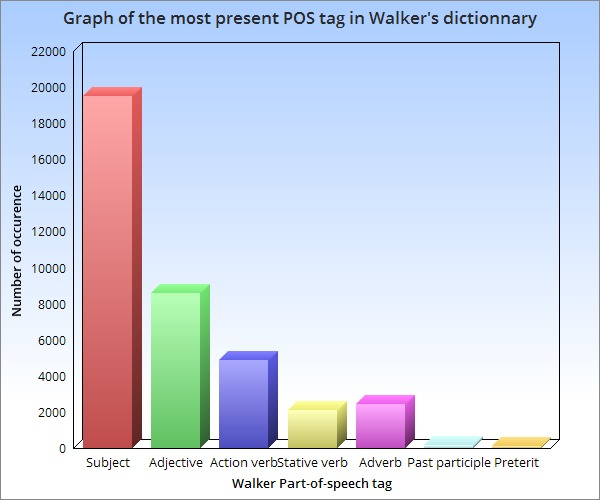
\includegraphics[width=8cm]{tagsetChart.jpeg}\\

\vspace{2mm}

Walker used many tags as Part-Of-Speech tags but the Brown Corpus doesn't consider all of them:
for e.g. there are no  \textit{plural, contraction} or \textit{A negative or privative termination.}\\

\vspace{2mm}

The word \textit{MEN} is tagged as \textbf{plural} but the word \textit{WOMEN} isn't.\\

\vspace{2mm}

The tag \textbf{contraction}  hasn't been used for every words which required it. For instance, the word \textit{NE'ER} is a poetical contraction for Never  and the word \textit{TA'EN} is a poetical contraction for Taken. While \textit{NE'ER} is declared as an adverb, \textit{TA'EN} is declared as a contraction.

\end{center}
